\documentclass[12pt]{article}
\usepackage{amsthm,amssymb,amsmath,amsfonts}
\usepackage[a4paper, top=25mm, bottom=30mm, left=25mm, right=25mm]{geometry}
\usepackage[pagebackref=false,colorlinks,linkcolor=black,citecolor=black]{hyperref}
\usepackage[nameinlink]{cleveref}
 \AtBeginDocument{%
    \crefname{equation}{برابری}{equations}%
    \crefname{chapter}{فصل}{chapters}%
    \crefname{section}{بخش}{sections}%
    \crefname{appendix}{پیوست}{appendices}%
    \crefname{enumi}{مورد}{items}%
    \crefname{footnote}{زیرنویس}{footnotes}%
    \crefname{figure}{شکل}{figures}%
    \crefname{table}{جدول}{tables}%
    \crefname{theorem}{قضیه}{theorems}%
    \crefname{lemma}{لم}{lemmas}%
    \crefname{corollary}{نتیجه}{corollaries}%
    \crefname{proposition}{گزاره}{propositions}%
    \crefname{definition}{تعریف}{definitions}%
    \crefname{result}{نتیجه}{results}%
    \crefname{example}{مثال}{examples}%
    \crefname{remark}{نکته}{remarks}%
    \crefname{note}{یادداشت}{notes}%
    \crefname{observation}{مشاهده}{observations}%
    \crefname{algorithm}{الگوریتم}{algorithms}%
    \crefname{cproof}{برهان}{cproofs}%
}

\usepackage{tikz}
\usepackage{graphicx}
\usepackage{booktabs}
\usepackage{color}
\usepackage{graphicx}
\usepackage{subcaption}

\usepackage{setspace}
\doublespacing

\usepackage{titletoc}
\usepackage{tocloft}
\usepackage{enumitem}
\usepackage{amsmath, amssymb}
\usepackage{algorithm}
\usepackage[noend]{algorithmic}
\renewcommand{\algorithmicrequire}{\textbf{Input:}}
\renewcommand{\algorithmicensure}{\textbf{Output:}}

\usepackage{tabularx}
\makeatletter
\newcommand{\multiline}[1]{%
  \begin{tabularx}{\dimexpr\linewidth-\ALG@thistlm}[t]{@{}X@{}}
    #1
  \end{tabularx}
}
\makeatother

\usepackage{float}
\usepackage{verbatim}
\makeindex
\usepackage{sectsty}
\usepackage{xepersian}
\SepMark{-}
\settextfont[Scale=1.2,Path=fonts/,BoldFont=B Nazanin Bold.ttf]{B Nazanin.ttf}
\setlatintextfont{Times New Roman}
\renewcommand{\labelitemi}{$\bullet$}

\theoremstyle{definition}
\newtheorem{definition}{تعریف}[section]
\newtheorem{remark}[definition]{نکته}
\newtheorem{note}[definition]{یادداشت}
\newtheorem{example}[definition]{نمونه}
\newtheorem{question}[definition]{سوال}
\newtheorem{remember}[definition]{یاداوری}
\newtheorem{observation}[definition]{مشاهده}
\theoremstyle{theorem}
\newtheorem{theorem}[definition]{قضیه}
\newtheorem{lemma}[definition]{لم}
\newtheorem{proposition}[definition]{گزاره}
\newtheorem{corollary}[definition]{نتیجه}
\newtheorem*{cproof}{برهان}




\begin{document}
\fontsize{12pt}{14pt}\selectfont

\begin{minipage}{0.1\textwidth}

\includegraphics[width=3cm]{etc/IUST}
\end{minipage}%
\hfill%
\begin{minipage}{0.6\textwidth}\centering
\fontsize{13pt}{13pt}\selectfont
به‌ نام خدا \\
\textbf{درس یادگیری عمیق} \\
\textbf{تمرین سری ششم}\\
استاد درس : دکتر محمدرضا محمدی \\
دستیاران :  مهدی خورشا، سید محمد موسوی،\\ امیرحسین نمازی
\\
\vspace{0.25cm}
\begingroup
\fontsize{11pt}{11pt}\selectfont
دانشگاه علم و صنعت ایران، دانشکده مهندسی کامپیوتر \\
نیمسال دوم تحصیلی 1403 - 1404 \\
\endgroup
\end{minipage}%
\hfill%
\begin{minipage}{0.1\textwidth}

\end{minipage}

\vspace{0.5cm}

\noindent\rule{\textwidth}{1pt}

\centering {\fontsize{18}{22}\selectfont \textbf{مهلت تحویل : 1404/01/15 }}\\
{\fontsize{14}{22}\selectfont \textbf{لطفا به نکات موجود در سند قوانین انجام و تحویل تمرین ها دقت فرمایید. }}

\begin{enumerate}

    \section*{سوالات تئوری}
    \item 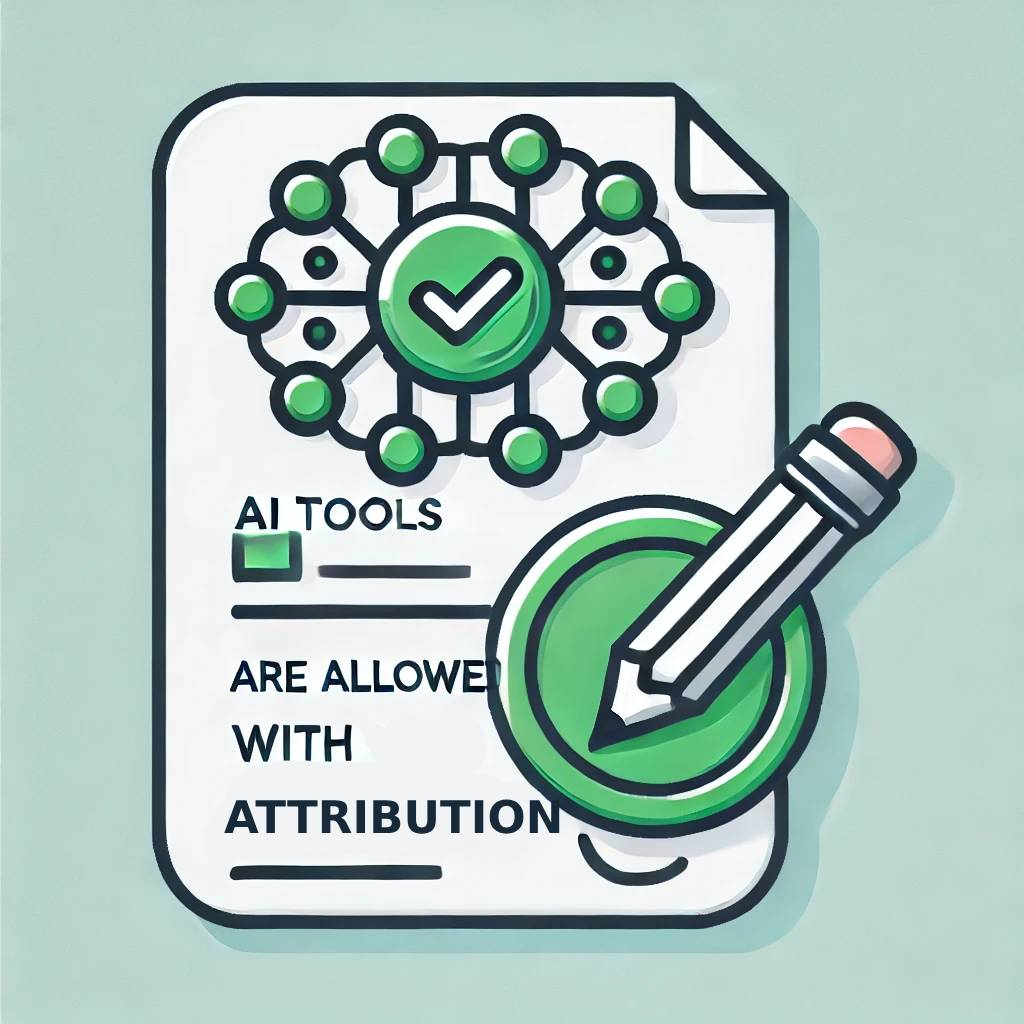
\includegraphics[width=1cm]{figs/Allowed_with_contributino.jpg}
     ابتدا مقاله \href{https://arxiv.org/pdf/2208.03608}{\lr{Shap-CAM}} را مطالعه کنید و سپس به سوالات زیر پاسخ دهید(10نمره).\\
     \begin{enumerate}
         \item روش‌های \lr{Grad-CAM} و \lr{Shap-CAM} را از نظر ویژگی‌های زیر مقایسه کنید:
         \begin{itemize}
             \item نحوه محاسبه اهمیت ویژگی‌ها (ویژگی‌های محلی یا جهانی)
             \item وابستگی به ساختار مدل و نیاز به گرادیان
             \item دقت در شناسایی نواحی مهم تصویر
             \item حساسیت به تغییرات کوچک در ورودی
         \end{itemize}
         \textbf{برای پاسخ به این بخش میتوانید از این \href{https://arxiv.org/pdf/2412.16003}{مقاله} استفاده کنید.}
         \vspace{1cm}
         \item فرض کنید مدلی که برای طبقه‌بندی تصاویر استفاده می‌کنید، نسبت به تغییرات ناچیز در ورودی حساس است.
         \begin{itemize}
             \item آیا انتظار دارید \lr{Grad-CAM} و \lr{Shap-CAM} رفتار مشابهی داشته باشند؟ چرا؟
             \item کدام روش می‌تواند پایداری بیشتری داشته باشد؟ توضیح دهید.
         \end{itemize}
     \end{enumerate}
     \vspace{1cm}

    \item 
\includegraphics[width=1cm]{figs/Forbidden_AI.jpg}
    به سوالات زیر در مورد شبکه های عصبی پیچشی\LTRfootnote{Convolutional} پاسخ دهید(10 نمره)\\
    \begin{enumerate}
        \item مفهوم به اشتراک‌گذاری پارامترها در شبکه‌های عصبی پیچشی چیست و چه تاثیری در روند آموزش مدل دارد؟
        \item توضیح دهید برای هریک از سناریوهای زیر شبکه‌های عصبی پیچشی مناسب هستند یا خیر:
        \begin{itemize}
            \item نظارت بر یک گونه‌ی خاص از گرگ در حیات وحش با پهپاد
            \item استخراج متن از درون صوت
            \item شناسایی عمل انجام شده درون ویدیو
            \item داوری انجام حرکت میل‌زنی در مسابقات زورخانه‌ای
        \end{itemize}
        \item معادله‌ی تلفیق (\lr{fusion}) لایه‌ی \lr{batchNorm2D} درون یک لایه‌ی \lr{Conv2D} را بنویسید و توضیح دهید این عمل چه تاثیری در عملکرد مدل دارد.
        \item یکی از کاربردهای مدل‌های چندوجهی\LTRfootnote{Multi-Modal}  مانند \lr{ChatGPT} وظیفه‌ی \lr{VQA}\LTRfootnote{Visual question answering}  (پرسش و پاسخ تصویر) است. در این وظیفه مدل تصویر و سوالی درباره‌ی تصویر از کاربر می‌گیرد و باید جواب متناسبی برای آن تولید کند. یکی از نقاط ضعف این مدل‌ها، پاسخ دادن به سوالاتی است که از جزئیات ریز و درحاشیه‌ی تصویر پرسیده می‌شوند. این نوع مدل‌ها در پاسخ به سوالات مربوط به تصویر حاوی یک شی برجسته در وسط توانایی خوبی دارند. برای پوشش دادن این ضعف یکی از کارهایی که می‌توان کرد، تشخیص درست ناحیه‌ی مورد پرسش و برش آن برای ورود به مدل است. فرض کنید ما یک مدل \lr{Question-image matching} توسعه داده‌ایم. اما این مدل تنها میان مفهوم کلی سوالات ورودی و تصویر انطباق انجام می‌دهد و درباره‌ی ناحیه‌ی آن اشاره‌ای نمی‌کند. با استفاده از مفاهیمی که تاکنون خوانده‌اید راه‌حلی برای این مسئله پیشنهاد دهید.
    \end{enumerate}
    \newpage
    \item 
\includegraphics[width=1cm]{figs/Forbidden_AI.jpg}
    تعداد پارامتر، ضرب و جمع و هم‌چنین میدان دید موثر لایه‌های شبکه‌ی عصبی با ورودی تصاویر رنگی از ابعاد 256 در 256 زیر را به تفصیل محاسبه کنید (لطفا اعداد اعشاری را به پایین گرد کنید)(15 نمره)\\
    
        \lr{
        {\ttfamily  
            \begin{itemize}
                \item \textbf{Layer1 : nn.Conv2d(in\_channels=3, out\_channels=32, kernel\_size=(7,7), stride=1, padding='same')}
                \item \textbf{bn1 : nn.BatchNorm2d(32)}
                \item \textbf{Layer2 : nn.Conv2d(in\_channels=32, out\_channels=64, kernel\_size=(5,5), stride=2, padding='valid')}
                \item \textbf{bn2 : nn.BatchNorm2d(64)}
                \item \textbf{Layer3 : nn.AvgPool2d(kernel\_size=(2,2), stride=2)}
                \item \textbf{Layer4 : nn.Conv2d(in\_channels=64, out\_channels=128, kernel\_size=(3,3), stride=1, dilation=2, padding='valid')}
                \item \textbf{bn3 : nn.BatchNorm2d(128)}
                \item \textbf{Layer5 : nn.Conv2d(in\_channels=128, out\_channels=128, kernel\_size=(3,3), stride=1, dilation=1, padding='valid')}
                \item \textbf{bn4 : nn.BatchNorm2d(128)}
                \item \textbf{Layer6 : nn.AvgPool2d(kernel\_size=(2,2), stride=2)}
                \item \textbf{Layer7 : nn.Conv2d(in\_channels=128, out\_channels=256, kernel\_size=(3,3), stride=1, padding='valid')}
                \item \textbf{bn5 : nn.BatchNorm2d(256)}
                \item \textbf{Layer8 : nn.AvgPool2d(kernel\_size=(2,2), stride=2)}
                \item \textbf{fc1 : nn.Linear(in\_features=43264, out\_features=1024)}
                \item \textbf{fc2 : nn.Linear(in\_features=1024, out\_features=1024)}
                \item \textbf{dropout : nn.Dropout(p=0.5)}
                \item \textbf{fc3 : nn.Linear(in\_features=1024, out\_features=10)}
            \end{itemize}
            } }
    
       
    \section*{سوالات عملی} 
    \item 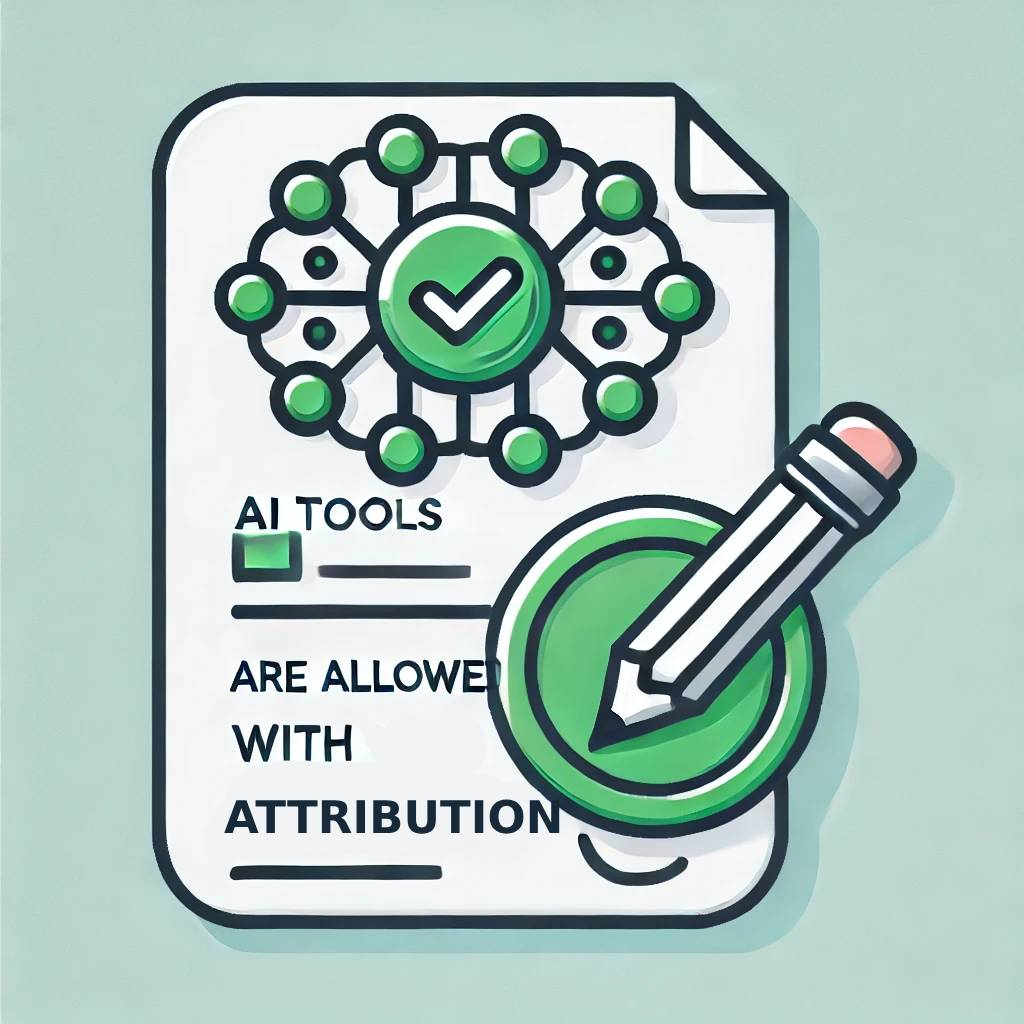
\includegraphics[width=1cm]{figs/Allowed_with_contributino.jpg}
    برای انجام این سوال به پوشه‌ی \lr{HW2\_TM} مراجعه کرده و درون فایل نوتبوک پیوست شده، سعی کنید جاهای خالی را پر کنید. برای این سوال از تصاویری که درون همان پوشه قرار داده شده‌اند استفاده کنید.\\
    در این سوال به یکی از مسائل مهم بینایی کامپیوتر به نام تطبیق کلیشه پرداخته‌ایم. در این مسئله دو نوع ورودی به نام‌های تصویر کلیشه و تصویر جست‌وجو داریم که هدف یافتن تصویر کلیشه درون تصویر جست‌وجو و برجسته‌سازی آن با رسم مستطیل به دور شی یافته شده است. یکی از ابتدائی‌ترین روش‌های انجام این مسئله این است که تصویر جست‌وجو را به نواحی‌ای تقسیم‌بندی کرده و شباهت هر یک را با تصویر کلیشه بسنجیم. اما انجام این کار دارای چالش‌های فراوانی است اعم از: کند بودن فرایند، احتمال وجود تغییرات زیاد میان کلیشه و جست‌وجو و ... . از این رو روش های مبتنی بر شبکه‌های عصبی پیچشی برای این مسئله پیشنهاد شدند که دارای دقت عملکردی بالا در مدت زمان معقولی بودند.\\
    بیشتر کد درون نوتبوک برای شما به‌صورت آماده آورده شده است. هدف از این سوال این است که آن را مطالعه کنید و درون گزارشی توضیح دهید که شبکه‌های عصبی پیچشی درون این کد چگونه به حل این مسئله کمک کرده‌اند (از آوردن جزئیاتی مانند: نحوه‌ی محاسبه‌ی \lr{confidence}، توابع کمکی، توابع رسم نتایج، \lr{NMS} و ... بپرهیزید و تنها اشاره کنید شبکه‌های عصبی پیچشی چگونه دقت و سرعت این مسئله را افزایش داده‌اند)\\
    خرجی‌های مورد انتظار درون نوتبوک فراهم شده‌اند(15 نمره).

    \item 
\includegraphics[width=1cm]{figs/Forbidden_AI.jpg}
    در این سوال قرار است برای مجموعه‌ی داده‌ی زیر برای شناسایی اعداد دست‌نویس از روی تصویر ورودی، یک شبکه‌ی عصبی پیچشی با معماری دلخواه توسعه دهید. تصاویر این مجموعه‌داده، تصاویر رنگی 64 در 64 تایی از اعداد انگلیسی 1 تا 4 هستند که باید توسط شبکه‌های عصبی پیچشی آن‌ها را شناسایی کنند. این تصاویر برچسب ندارند و از روی اسم هر فایل باید ساخته شود. در شکل \ref{fig:num_pic} نمونه‌ای از این تصاویر برای شما آورده شده است(15 نمره)\\
    
    \begin{figure}[h]
        \centering
        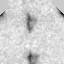
\includegraphics[width=1cm]{figs/num_pic.jpg}
        \caption{نمونه ای از تصویر عدد 4}
        \label{fig:num_pic}  
    \end{figure}

    
    می‌توانید برای این مجموعه‌داده رویه‌های مختلف داده‌افزایی را اعمال کنید.\\
    برای انجام آن به نوتبوک \lr{HW2\_CNN.ipynb} که به‌همراه سوالات پیوست گردیده است رجوع کرده و درون آن سعی کنید نواحی خالی را پر کنید.\\
    در این سوال انتظار می‌رود بتوانید مدلی را توسعه دهید که برای مجموعه‌داده‌ی آموزشی و آزمایشی (با نرخ 80 به 20 درصد از کل مجموعه‌داده با \lr{random seed = 42} برای جداسازی) به دقت بالای 90 درصد دست یابید.
    لطفا ابرپارامترهای مورد نیاز را برای احقاق نیازمندی‌های پروژه تنظیم کنید.\\
    در معماری مدل مختار هستید و می‌توانید از هر نوع مدلی استفاده کنید.\\
    پیشنهاد می‌شود از \lr{callback} هایی مانند \lr{early stopping} و \lr{learning rate scheduler} برای بهبود روند آموزش مدل استفاده کنید. (در استفاده نکردن از آن‌ها آزاد هستید.)\\
    \textbf{درون نوتبوک رویه‌ی ساخت برچسب واقعی برای هر تصویر برای شما پیاده‌سازی شده است.}\\
    \href{https://drive.google.com/drive/folders/1B66Pref_4TTUszYh5Tb08udCIIphXkl9?usp=sharing}{لینک مجموعه داده}


    \item 
\includegraphics[width=1cm]{figs/Allowed_recommended.jpg}
    مقاله \href{https://arxiv.org/pdf/1611.05431}{\lr{ResNeXt}} را مطالعه کنید و سعی کنید به دلیل موفقیت خلاقیت به کار رفته در آن خوب فکر کنید. در این سوال میخواهیم یک بلاک مشابه بلاک معرفی شده در مقاله پیاده سازی کرده و به کمک آن یک شبکه کامل بسازیم و سپس آنرا با دیتاست \lr{cifar100} آموزش دهیم.\\
    به نوتبوک \lr{Resnext.ipynb} مراجعه کنید. ابتدا یک کلاس برای بلاک \lr{resnext} طراحی کنید. سپس یک کلاس برای طراحی کامل شبکه بنویسید.در این بخش نه تنها نیازی نیست به شبکه های معرفی شده در مقاله(مانند \lr{resnext29}) وفادار باشید، بلکه توصیه میشود در طراحی خلاقیت خود را به کار بگیرید. در ساماندهی شبکه مادامی که به ایده اصلی مقاله پایبند باشید پیاده سازی شما مورد قبول است.\\
    در قسمت بعد پیش پردازش مناسب روی داده ها انجام دهید و دیتا لودرهای مورد نیاز خود را بسازید. در این قسمت تمام دانشی که در کلاس درس دراین مورد به دست آورده اید به کار بگیرید. در قسمت بعد آموزش مدل را شروع کنید. مدیریت نرخ یادگیری، نگهداری بهترین مدل و رگولاریزیشن مناسب از جمله مواردی هستند که باید به آنها توجه کافی داشته باشید. در قسمت پایانی دقت مدل را روی مجموعه دادگان تست اندازه گرفته و گزارش کنید(15 نمره).\\
    \textbf{توجه : تسلط شما به مقاله و ایده آن در زمان ارایه سنجیده خواهد شد و نیازی به گزارش نویسی برای آن نیست.}
    
    \item 
\includegraphics[width=1cm]{figs/Allowed_recommended.jpg}
    در این تمرین قصد داریم به مصورسازی آنچه یک شبکه پیش آموخته در مورد یک کلاس خاص فکر میکند بپردازیم. در کلاس درس یک روش برای بهینه سازی ورودی به قصد تولید تصویر بیشینه کننده احتمال تعلق به یک کلاس برای شبکه های پیش آموخته معرفی شد. در صورت نیاز به جزییات بیشتر در مورد این روش میتوانید به این \href{https://yosinski.com/deepvis}{لینک} مراجعه کنید. در این روش ابتدا یک کلاس(مثلا فلامینگو) را در نظر میگیرید و با شروع از یک تصویر تصادفی و بهینه سازی آن به تصویری میرسید که شبکه آن را متعلق به کلاس مربوطه بداند.\\
    در قسمت دوم سوال قصد داریم با استفاده از حمله \lr{fgsm} تصویری را که به نظر ما و شبکه متعلق به یک کلاس است را با کمترین تغییر به تصویری تبدیل کنیم که به نظر شبکه متعلق به کلاس مورد نظر نباشد. در صورت نیاز میتوانید این لینک را درمورد حمله \href{https://medium.com/@zachariaharungeorge/a-deep-dive-into-the-fast-gradient-sign-method-611826e34865}{\lr{fgsm}} مطالعه کنید.\\
    یک کلاس مشخص برای هر دوقسمت سوال در نظر بگیرید و تصویر به دست آمده از دو بخش را باهم مقایسه کنید(20 نمره).

    \section*{سوال امتیازی} 
    \item 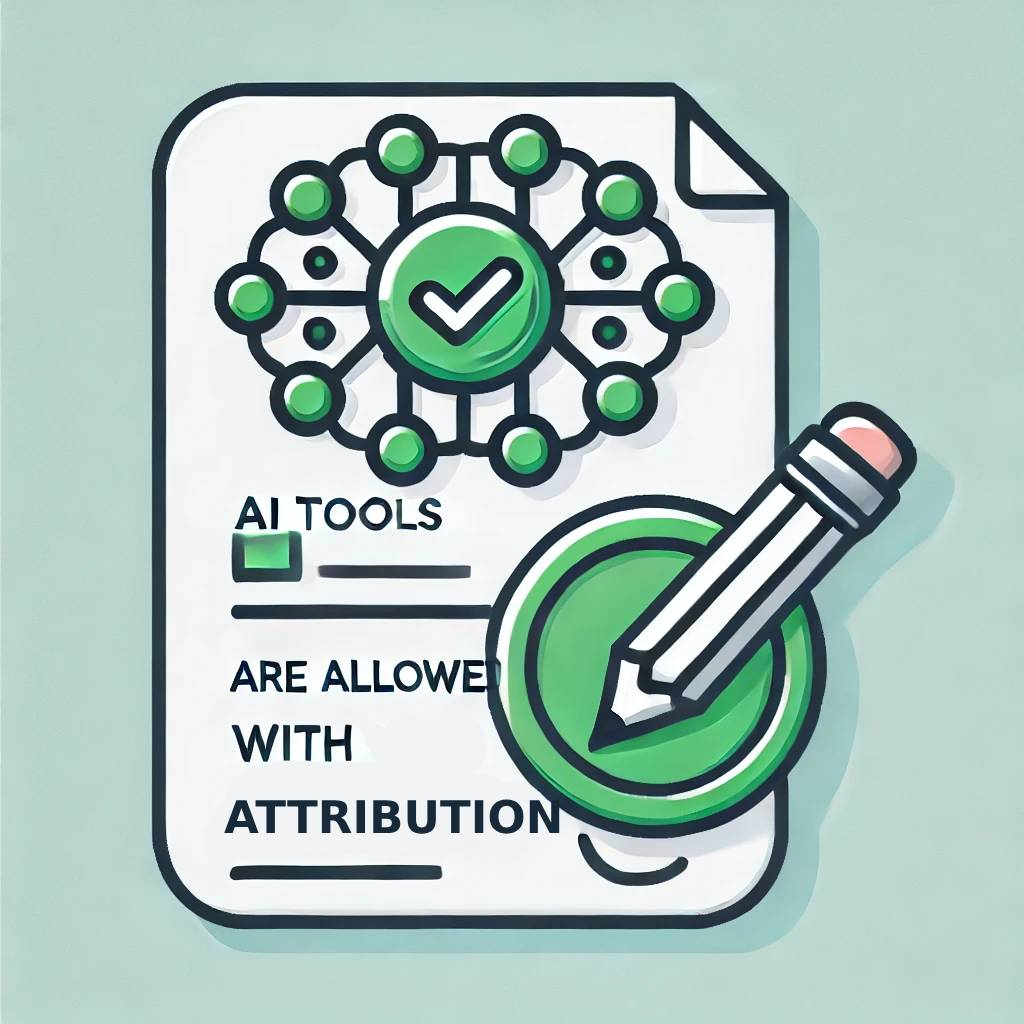
\includegraphics[width=1cm]{figs/Allowed_with_contributino.jpg}
    در این سوال قصد داریم یک مدل ناحیه‌بند معنایی  برای تصاویر \lr{X-Ray} موجود برای شناسایی نواحی پوسیدگی دندان توسعه دهیم. مسئله‌ی ناحیه‌بندی معنایی یکی از شناخته‌شده‌ترین مسائل بینایی کامپیوتر می‌باشد که در آن هدف دسته‌بندی تمامی پیکسل‌های موجود در تصویر است. شبکه‌های عصبی پیچشی با ساختاری خاص نشان‌داده‌اند که دارای قدرت مناسبی برای حل این مسئله هستند. مدل‌های \lr{SS} انواعی از شبکه‌های عصبی پیچشی هستند که ابتدا تصویر ورودی را رمزگذاری  می‌کنند تا بتوانند ویژگی‌های مناسب از تصویر ورودی را استخراج کنند. سپس در رویه‌ای به نام رمزگشایی  از روی ویژگی‌های ساخته شده، سعی می‌کنند به فضای اولیه‌ی تصویر ورودی (با همان ابعاد یکسان) بازگردند و پیکسل‌های تصویر را دسته‌بندی می‌کنند. یکی از انواع موفق شبکه‌های عصبی پیچشی در این حوزه، مدل‌های \href{https://arxiv.org/pdf/1505.04597}{\lr{Unet}} می‌باشند که ابتدا به‌صورت تدریجی تصویر را رمزگذاری کرده و سپس به‌صورت تدریجی ابعاد ویژگی‌های استخراج شده را به ابعاد تصویر اولیه بازمی‌گردانند تا عملیات دسته‌بندی را انجام دهند و در این میان تعداد مشخصی ارتباط میان رمزگذار و رمزگشا برقرار می‌کند تا بتواند از ویژگی‌های سطح پایین در این مسئله بهره ببرد. در این مسئله برچسب ورودی تصویر هم بعد تصویر ورودی با تعداد چنل 1 است که مقدار پیکسل‌های آن نشان‌دهنده‌ی کلاس آن پیکسل می‌باشد. از موارد کاربرد این مدل‌ها می‌توان به مسائل پزشکی و یافتن نواحی دارای تومور، پوسیدگی و ... از روی تصاویر پزشکی اشاره کرد.\\
    در این سوال نوع خاصی از مدل \lr{Unet} به نام \lr{ResUNet} در نظرگرفته شده است. این مدل ساختار یکسانی با مدل \lr{Unet} اصلی داراست با این تفاوت که رمزگذار آن یک مدل پیچشی \lr{Residual} است (دارای ارتباطات \lr{residual} درون رمزگذار است.). به نوتبوک \lr{HW2\_SS.ipynb} رجوع کرده و تلاش کنید با پر کردن جاهای خالی این وظیفه را به درستی پیاده‌سازی کنید.\\
    در نظر داشته باشید که از مدل فوق تنها قسمت رمزگذار آن از شما خواسته شده و باقی قسمت‌های مدل برای شما پیاده‌سازی شده‌اند.\\

    مجموعه‌داده‌ی این مسئله درون نوتبوک قرار داده شده است و با اجرای سل مربوط، مجموعه‌داده برای شما دانلود خواهد شد. اما در نظر داشته باشید که برخی از برچسب‌های این مجموعه‌داده به شدت نویزی شده‌اند که می‌تواند روند آموزش مدل شما را با مشکل روبرو کنند. برای مدیریت آن‌ها رویه‌ی متناسبی در نظر بگیرید.\\

    سعی کنید تابع هزینه (\lr{loss function}) مناسبی برای این مسئله توسعه دهید. این مسئله دسته‌بندی هر پیکسل میان دو کلاس (0 یعنی پوسیده نیست و 1 یعنی پوسیده هست) می‌باشد. یکی از توابع هزینه‌ی مناسب برای این کار \lr{BCE} می‌باشد و برای این نوع مسائل نیز استفاده می‌شود. اما استفاده از آن باید برای این مسئله بهینه شود (استفاده از تابع هزینه‌ی \lr{BCE} اولیه و بدون تغییر جواب خوبی نخواهد داد). (برای استفاده از سایر توابع هزینه‌ای که در کلاس تدریس نشده‌اند حتما منبع آن را ذکر کنید.)\\

    رسیدن به \href{https://oecd.ai/en/catalogue/metrics/dice-score#:~:text=The%20Dice%20score%20ranges%20from,of%20elements%20in%20set%20B)}{\lr{dice score}} بالای 40 درصد هم برای تصاویر آموزشی و هم آزمایشی الزامی است(20 نمره).\\
    

\end{enumerate}



\end{document}


